\documentclass[10pt, a4paper]{article}
\usepackage[margin=1in]{geometry}
\usepackage{cmbright}
\usepackage[OT1]{fontenc}
\usepackage{authblk}
\usepackage{siunitx}
\usepackage{babel,csquotes,xpatch}
\usepackage[backend=biber, style=numeric]{biblatex}
\usepackage{multicol}
\usepackage{amsmath}
\usepackage{enumitem}
\usepackage{booktabs}
\usepackage[hidelinks]{hyperref}
\usepackage{array}
\usepackage[normalem]{ulem}
\usepackage{tabularx}
\usepackage[labelfont=bf, textfont=normalfont, justification=raggedright, singlelinecheck=false, font=small]{caption}
\usepackage{float}
\usepackage{titlesec}
\titleformat{\section}
  {\normalfont\bfseries}
  {\thesection}{1em}{} 
\titlespacing*{\section}{0pt}{1.2\baselineskip}{0.6\baselineskip}
\titleformat{\subsection}
  {\normalfont\itshape} 
  {\thesubsection}{1em}{} 
\titlespacing*{\subsection}{0pt}{1\baselineskip}{0.4\baselineskip}
\DeclareSIUnit\mmHg{mmHg}
\DeclareSIUnit\bar{bar}
\usepackage{tikz}
\usetikzlibrary{positioning, arrows.meta, matrix, calc}
\usepackage{circuitikz}
\usepackage{graphicx}
\usepackage{wrapfig}
\addbibresource{gm1_short_team_report.bib}
\title{
    Short Team Report\\[0.5em] 
    \Large Team 2: Low Cost Perfusion Pump\\[0.25em]  
    \normalsize Part IIA: \texttt{GM1} \textit{Multidisciplinary Design}
}

\author[1]{Tahmid Azam}
\author[1]{Luca Buxton}
\author[1]{India Henry}
\author[1]{Lonnie McKiernan}
\author[1]{Lucy Payne}

\affil[ ]{{\normalsize Mentored by Dr. Peter Long and Prof. Athina E. Markaki}}
\affil[ ]{{\small}}
\affil[1]{Department of Engineering, University of Cambridge}

\date{20 March 2026}

\begin{document}
\maketitle

\begin{abstract}
    The bioengineering department are investigating the applications of collagen-based synthetic blood vessels for haemodialysis, involving the measurement of vessel compliance under different pressure profiles. The existing peristaltic pump setup suffers from poor pressure sensor dynamic range, unwanted pressure pulsations requiring extensive compliance tubing, and non-physiological pulse rates. We propose a dual-syringe pump system driven by stepper motors and lead screws, with voice coil actuators or pinch valves to superimpose a physiological AC waveform onto a steady DC pressure baseline. A PID-based control system running on an ESP32 microcontroller enables real-time waveform tracking, with software providing both GUI and CLI interfaces for experiment configuration and data logging. The estimated prototype cost is under \SI{210}{\pounds}, with a final product target of \SIrange{50}{100}{\pounds}, offering a low-cost, reproducible alternative suitable for parallel graft testing.
\end{abstract}

\newpage

\section{Clinical motivation}

Haemodialysis is the process of removing blood from the body, passing it through a dialyser which filters it, and then returning it to the body, and is indicated in cases of kidney failure.
The department is looking to penetrate the artifical vessel graft market by targeting an application that doesn't pose immediate threat to life upon failure (in contrast to grafts for bypass surgery, e.g. coronary bypass), involves use on much shorter timescales, and features simpler medical device regulation.
In order to support the high flow rates required for haemodialysis ($>\SI{300}{\milli\liter\per\minute}$), arteriovenous (AV) fistulas are commonly surgically formed.
In the elderly population, the formation of AV fistulas can be more challenging due to vessel damage from natural and iatrogenic causes (e.g., repeated blood samples over many years), as well as slow time to maturation \supercite{mcgroganArteriovenousFistulaOutcomes2015}.
Synthetic vessel grafts help form a AV fistula with a shorter maturation period, or for patients with exhausted vascular access sites \supercite{akohProstheticArteriovenousGrafts2009}.
In the case of artificial vessels for uses in bypass grafts, they offer greater availability over the current sources of donor vessels from the great veins of the leg, which may be damaged and require modification in order for arterial applications.

\section{Existing laboratory setup and its limitations}

\begin{figure}[H]
    \resizebox{\textwidth}{!}{%
        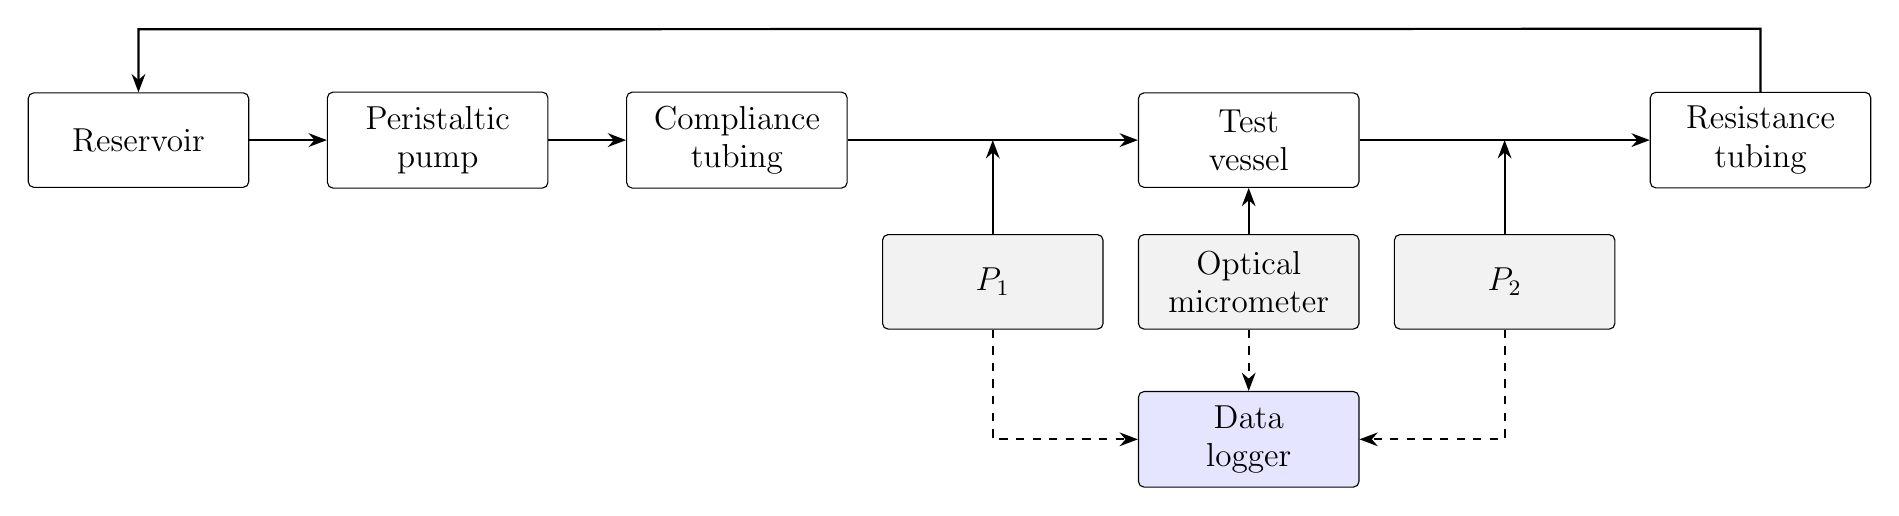
\begin{tikzpicture}[
                box/.style={draw, rounded corners=2pt, minimum height=12mm, minimum width=28mm, align=center, inner sep=5pt, font=\large},
                sensor/.style={box, fill=gray!10},
                logger/.style={box, fill=blue!10},
                arr/.style={-Stealth, thick},
                sig/.style={-Stealth, dashed, thick},
            ]

            % Main circuit:
            \node[box] (res)  at (0,   0) {Reservoir};
            \node[box] (pump) at (3.8, 0) {Peristaltic\\pump};
            \node[box] (rt1)  at (7.6, 0) {Compliance\\tubing};
            \node[box] (ves)  at (14.1, 0) {Test\\vessel};
            \node[box] (rt2)  at (20.6, 0) {Resistance\\tubing};

            % Flow arrows with the return loop going over the top:
            \draw[arr] (res) -- (pump);
            \draw[arr] (pump) -- (rt1);
            \draw[arr] (rt1) -- (ves);
            \draw[arr] (ves) -- (rt2);
            \draw[arr] (rt2.north) -- ++(0,0.8) -- ($(res.north)+(0,0.8)$) -- (res.north);

            % Pressure sensor taps with sensors below the main flow and arrows pointing toward flow line:
            \coordinate (tap1) at ($(rt1.east)!0.5!(ves.west)$);
            \coordinate (tap2) at ($(ves.east)!0.5!(rt2.west)$);
            \node[sensor] (p1) at ($(tap1)+(0,-1.8)$) {$P_1$};
            \node[sensor] (p2) at ($(tap2)+(0,-1.8)$) {$P_2$};
            \draw[arr] (p1.north) -- (tap1);
            \draw[arr] (p2.north) -- (tap2);

            % Optical micrometer below the vessel, arrow pointing toward vessel:
            \node[sensor] (mic) at ($(ves)+(0,-1.8)$) {Optical\\micrometer};
            \draw[arr] (mic.north) -- (ves.south);

            % Data logger below sensors:
            \node[logger] (dl) at ($(ves)+(0,-3.8)$) {Data\\logger};

            % Signal lines:
            \draw[sig] (p1.south)  |- (dl.west);
            \draw[sig] (p2.south)  |- (dl.east);
            \draw[sig] (mic.south) -- (dl.north);
        \end{tikzpicture}
    }
    \caption{Existing laboratory bench setup.}
    \label{fig:existing_bench}
\end{figure}

\autoref{fig:existing_bench} displays the current laboratory setup bench setup of the perfusion system. The current pump being used is a Kamoer KK1800 peristaltic pump, which uses rollers to occlude sections of the tubing, pushing fluid through the system. This then passes through a section of compliance tubing, to smooth out any pulsations from the peristaltic pump. The flow then enters the perfusion chamber, where the pressure is measured either side of the collagen graft using 100 psi-rated pressure sensors. An optical micrometer is used to monitor diameter changes of the graft, in order to ascertain the average compliance of the grafts. Resistance tubing is required downstream of the test section in order to create a back pressure to set the mean pressure of the flow. The silicone tubing used through the pump  has an outer diameter of 8mm, which feeds into tubing of 5mm outer diameter. We have identified some key problem areas of this testing setup:
\begin{itemize}[noitemsep]
    \item The pressure sensors used in the current setup have a large atmospheric pressure offset, resulting in wasted dynamic range.
    \item The peristaltic pump creates unwanted pressure spikes, so 5 metres of compliance tubing are currently used -- this creates a cluttered workspace and a suboptimal way of replicating a physiological pressure profile.
    \item Achieving flow rates of up to 400mL/min requires un-physiologically large pulse rates of approximately 570 BPM.
\end{itemize}

\section{Design brief}


In order to tackle the three problems found in the laboratory setup, a specification list for our pump has been produced. Each requirement has been classified as high or low value depending on how much risk it involves and how essential it is to the product functionality.

\begin{table}[H]
    \small
    \centering
    \begin{tabularx}{\linewidth}{>{\raggedright\arraybackslash}p{4.5cm} p{2cm} X}
        \toprule
        \textbf{requirement} & \textbf{value}                                                                        & \textbf{rationale} \\
        \midrule

        Semi-continuous operation
                             & High
                             & Allows for longer testing of grafts, improving understanding of fatigue and leakage.                       \\

        Mean pressure of 80--120\,mmHg
                             & High
                             & Replicates physiological baseline arterial pressure.                                                       \\

        Flow remains uncontaminated
                             & High
                             & Enables continuous operation without requiring fluid replacement.                                          \\

        Prevent crushing of blood cells
                             & High
                             & Allows working fluid to be exchanged to blood.                                                             \\

        Compatible with a tubing outer diameter of 5\,mm
                             & Medium
                             & Improves physiological realism and compatibility with standard laboratory setups.                          \\

        Produce flow rates up to 400\,ml/min
                             & Medium
                             & Enables testing of dialysis-relevant flow rates at realistic heart rates.                                  \\

        Pressure controlled to replicate physiological pulse
                             & Medium
                             & Ensures collected data closely mimics in vivo flow conditions.                                             \\

        Run multiple pumps in parallel
                             & Low
                             & Allows simultaneous testing of multiple grafts.                                                            \\

        Replicate flows in different vessels
                             & Low
                             & Provides flexibility for different graft diameters and vessel types.                                       \\

        Display key parameters and allow for modification
                             & Low
                             & Enables user control of mean, systolic, and diastolic pressure, as well as flow rate.                      \\

        \bottomrule
    \end{tabularx}
    \caption{System requirements and rationale}
\end{table}

Following on from the development of the design requirements, the following problem statement was derived:
\begin{quote}
    ``Design a low-cost mechanical pump able to accurately replicate physiological flows.''
\end{quote}





\section{Proposed system overview}

\begin{wrapfigure}{r}{0.4\textwidth}
    \centering
    \includegraphics[width=0.38\textwidth]{../presentation-2026-03-18/images/design.jpg}
    \caption{The proposed dual-syringe design.}
    \label{fig:design}
\end{wrapfigure}

Given the project requirements and desired outputs, the most suitable, low cost design, while having sufficient control was decided to be a dual syringe pump system as shown in \autoref{fig:design}. Two syringes are to be connected up in parallel, each driven by a separate linear drive mechanism consisting of a stepper motor attached to a lead screw via a gearbox. Continuous flow will be generated with one syringe pushing fluid to the test grafts as the other pulls from the reservoir. There will be some overlap with the pushing cycles of the syringes, to avoid a large drop in pressure or flow rate. One-way valves will be placed at the exit of the syringes to prevent backflow, with additional voice coil actuators added downstream of the test region to throttle the flow. These actuators will act to adjust the constant DC pressure output by the syringes, to superimpose the non-standard waveform of the heartbeat. This fine control over the fluid allows closer matching of the physiological conditions of the heart, unlike the peristaltic pump in the original set-up. Two pressure sensors complete the initial design, either side of the test region providing readings for feedback control over the motors and actuators.

\section{Mechanical}

\subsection{Housing and assembly}

Ideally the entire pump will be reproducible to allow multiple pumps to be testing the grafts in parallel. This means the housing components need to be easily printed and assembled while maintaining a secure fit to avoid leakages and reduce backlash. Once the configuration of the fluid circuitry is set-up, the housing will be designed in SolidWorks based on these dimensions and 3-D printed. A strong printer filament is required to withstand repeated loading so PETG is recommended, with low brittleness ($>\qty{7}{\percent}$ elongation at yield \cite{PETGHFa}) and high bending strength ($>\qty{60}{\mega\pascal}$), over say PLA or Resin which would fracture easily under the applied loads. The housing will clamp the syringe and fix the gearbox and stepper motor, while allowing the moving carriage attaching the plunger to the lead screw, to translate vertically. Standard silicon tubing will be used throughout, with a \qtyrange{4}{5}{\milli\metre} internal diameter, using T-type connectors for the pressure sensors.

\subsection{Motors and drive system}

A stepper motor is well suited for this project due to its precise position control. While servo motors are an alternative, they are less cost-effective and require more complex PID control. To prevent continuous rotation at the end of each stroke, limit switches will be placed at both ends of the syringe to reverse the motor direction.
A lead screw, either directly coupled or geared, will be used to convert torque from the motor to linear force applied to the syringe. Achieving a flow rate of \qty{400}{\milli\litre\per\minute} requires a lead screw speed of \qty{\sim50}{RPM} (assuming a syringe diameter of \qty{3.56}{\centi\metre} and a pitch of \qty{8}{\milli\metre}, using the equation below). The theoretical plunger force is \qty{\sim1.6}{\newton}, corresponding to \qty{\sim0.0068}{\newton\metre} of torque, though friction between the plunger and barrel and misalignment of parts may increase this. Therefore, a NEMA~17 stepper motor with 200~steps/rev and a hold torque of \qty{0.17}{\newton\metre} has been chosen.
A key issue we predict arising is the motor may miss steps under high load, leading to position error and overshoot. This can be mitigated by increasing torque via a geartrain or a finer-pitch lead screw. For example, running the motor at \qty{500}{RPM} with a 10:1 reduction provides the required \qty{50}{RPM} while increasing torque by a factor of 10. This speed is within the range of operation of our chosen stepper motor. However, gearing introduces additional backlash, but this can be reduced using spring-loaded gears \cite{NonBacklashSpur}. The preliminary stage of development will require different lead screws and gear ratios to be tested in order to achieve the desired flow rates.

\subsection{Valves}

Further experimenting is required to determine which one-way valve configuration to use at the syringe exits. The first option is to use two cracking-pressure valves at a T-connection, placed in opposite directions. The precise cracking pressure does not need to be tightly specified, provided it is comfortably below the mean operating pressure of \qty{80}{\mmHg} (\qty{10.7}{\kilo\pascal}, or \qty{0.107}{\bar}). In practice, however, it would be preferable to select a cracking pressure somewhat below typical capillary pressures of \qty{20}{\mmHg} (\qty{2.7}{\kilo\pascal} or \qty{0.0267}{\bar}) to allow for potential future testing on various blood vessels. These check valves also help to mimic the physiological heart behaviours, with the semi-lunar valves opening at a certain pressure build up in the ventricles/atria. However more control can be brought to the design using instead a 3/2 valve which can be signalled to shut off flow to either the test grafts or from the reservoir. Therefore these can be timed exactly with the pushing of the plunger, but come at an expensive cost, typically 3x the price of check valves (\cite{PneumaticSolenoidValve}), so will be a fallback if the check valves are found to be unreliable in testing.

\subsection{Waveform generation}

In order to generate a physiological pressure profile, two methods were investigated. The key features to replicate are the systolic peak and dicrotic notch. Each method was assessed based on its ability to produce the systolic peak, requiring a pressure change of \qty{40}{\mmHg} (\qty{5.33}{\kilo\pascal}) over approximately \qty{0.1}{\second}.

The first method involves modulating syringe motion by varying the speed of the stepper motor. This changes the flow rate, which, according to Hagen--Poiseuille law, produces corresponding pressure variations. Equation \ref(below) estimates that a plunger displacement of \qty{\sim5}{\milli\metre} is required to achieve this pressure change. While this is a simplified calculation that neglects factors such as plunger friction and manufacturing tolerances, it highlights that the required motion is small, making precise control challenging and likely requiring iterative tuning. Reducing the syringe diameter could increase the required displacement and improve controllability.

The second method uses a pinch valve or voice coil actuator to partially occlude the tubing downstream of the test section. This increases flow resistance and therefore the pressure drop. Using Hagen--Poiseuille law, the required reduction in tube radius is calculated to be \qty{1.31}{\milli\metre}. This would require actuation at approximately \qty{10}{\hertz} with variable compression. A limitation is that pinch valves are typically binary, so a stiffer, thicker-walled tube may be needed to avoid complete occlusion. A voice coil actuator offers precise, high-speed displacement control, making it better suited for small, rapid compressions. This approach is also advantageous as it decouples the AC pressure component from the DC baseline pressure, allowing a wider range of physiological conditions (e.g.\ age, sex, cardiac health) to be simulated.

Therefore, a hybrid approach will be adopted. Both pinch valves and voice coil actuators will be evaluated initially. If the required precision proves difficult to achieve, a \qty{20}{\milli\litre} syringe may instead be used to inject pulsatile flow and replicate the desired physiological pressure profile.

\subsection{Pressure sensing}

\begin{table}[h]
    \small
    \centering
    \begin{tabularx}{\linewidth}{>{\raggedright\arraybackslash}p{4cm} p{3cm} X}
        \toprule
        \textbf{requirement} & \textbf{value}                                                                                    & \textbf{rationale} \\
        \midrule

        Operating range
                             & 80--120\,mmHg
                             & Physiological pressures in blood vessels.                                                                              \\

        Full range of sensor
                             & 150--500\,mmHg
                             & Provides burst tolerance and safety margin.                                                                            \\

        Sensor type
                             & Gauge
                             & Eliminates $\sim$760\,mmHg atmospheric offset, preserving dynamic range and improving resolution.                      \\

        System placement
                             & After AC and DC implementations
                             & Enables feedback control for both AC and DC components.                                                                \\

        Bandwidth
                             & 100\,Hz
                             & Supports a sampling frequency of 50\,Hz, sufficient to accurately track a $\sim$1\,Hz waveform.                        \\

        \bottomrule
    \end{tabularx}
    \caption{Pressure sensing requirements and rationale.}
\end{table}

\section{Software}

Through the software, laboratory personnel will be able to choose a pressure profile configuration and schedule of operation, view real-time pressure plots including the error for monitoring, and be able to log/export pressure data. For the lab environment, this would involve both a graphical user interface (GUI) for real-time visualisations and user-friendly changing of preferences and a command-line interface (CLI) for more advanced scripting for reproducible experiments and sharing of configurations, essential for peer-reviewed research. The software should be cross-platform, and support standard file formats for data export (e.g., comma-separated values, CSV). The software should be able to program schedules, such as a ramping mode of operation that slowly increases the pressure to find the bursting point. The software should also flag warnings for error states, such as sudden drops in pressure from a leak (e.g. vessel bursting) or sudden increases in pressure from a blockage (e.g., blockage from a clotting process). Cumulative error, percentage uptime at target pressure should also be monitored for evaluation. Storage demands involve \SI{2.34}{\kilo\byte\per\second} (3 \SI{64}{\bit} floats at \SI{100}{Hz}), with data transmitted over USB.

\subsection{Modelling the pressure profile}

There is huge variation in the pressure profile, and the software plans to offer multiple perspectives by which to model the cardiovascular system. Basic controls involve setting target systolic pressures, diastolic pressures, and heart rate. In addition, we can offer easier set up of experiment sets by incorporating normative data that adjusts these physiological variables for age \supercite{linIdentificationNormalBlood2016}, sex \supercite{joynerSexDifferencesBlood2016}, level of exercise \supercite{sharmanExerciseBloodPressure2015}, temperature, and the type of vessel (i.e., distance from the heart, such as artery, capillary, or venule). The chosen configuration and parameters can be exported, stored, or shared as JavaScript Object Notation (JSON) files for repeatability. The mathematical modelling of pressure profiles consists of splitting the target signal into two components: a constant mean DC pressure component, and an AC component. The DC component we model using the Windkessel model \supercite{westerhofArterialWindkessel2009} and literature values for the Womersley number for different vessel types, sensitive to the aging process \supercite{loudonUseDimensionlessWomersley1998}. The AC component we emulate by conducting Fourier analysis on literature representations of the cardiac cycle, to capture nuances such as the dicrotic notch.

\newpage
\section{Electrical}

\begin{wrapfigure}{r}{0.4\textwidth}
    \centering
    \includegraphics[width=0.38\textwidth]{images/elecdiagram.png}
    \caption{Electrical system diagram.}
\end{wrapfigure}

An ESP32 will be used, this will be cheaper and easier to scale compared to an arduino or RP. The display will be an alphanumeric display, anticipating that connecting the laptop may be more complicated than needed at the start. There will be a maximum of 4 stepper motor drivers. 2 will be used to push the syringes, and the other 2 will be used to open and close valves. These will be connected with general purpose I/O pins. Sensors will also be connected with GPIO. The computer will be connected through bluetooth, SPI, or other protocols like I2C, dependent on which is easiest. SPI will be attempted first. Power will be from the computer (5V) for the microcontroller, and from the wall with an adapter for the 12V needed for the motor driver.

\subsection{Timeline}

During week 1:
\begin{itemize}[noitemsep]
    \item hours 1-3: Create simple program, like turning on a light when a button is pressed to ensure microcontroller and software for mc - set up properly
    \item hours 3-5: connect stepper motor driver and motor, without syringe. Create simple code to test. Add syringe, and get power and pressure measurements.
    \item hours 5-6: connect display, ensure its working.
    \item hours 6-7: connect display to motor power.
    \item hours 7-10: connect and test sensors with water.
    \item hours 10-15: test multiple setups for pump, using different valves and placements of valves.
\end{itemize}
After this, the work needed to be done is less known. The best setup will be taken, and modelled in Python/MATLAB before being converted into hardware. Errors with sensing and motor control will be fixed.


\section{Control}
\subsection{Objectives and Constraints}
The primary objective of this control system is to track a continuously varying pressure waveform in real time, in order to make the pressure waveform received in the test vessel as close as possible to the reference pressure inputted. There is a hard constraint of the maximum safe pressure as vessel bursting is irreversible and expensive. However, the main challenge is handling the system nonlinearities. To name a few, the tubing compliance stores energy, the switching of syringes will create dead zones in the flow, the inertia of the fluid will create a lag, and the stepper motor is hard to keep track of and can slip.
\subsection{PID Controller Design}
Our solution to this is very fast sampling so that each control step can be approximated as linear. The system will filter (spec TBD) the raw sensor data, then a PID controller will map the error to a change in motor speed. PID control allows a response to current error, steady state offsets, and damping to prevent overshoots (burst constraint) \supercite{smuts2002pid}. The heart waveform is of the order of 1Hz and sampling frequency will be minimum 50Hz. DC and AC need to be controlled separately by motor speed and an AC actuator, the biggest challenge is to model exactly how changing the motor speed and the AC actuator changes the pressure. The PID will run on the microcontroller, and the gains will be initialised from calculations, then tuned manually as the mechanical setup is developed and tested. We may also explore feedforward to reduce lag, and to cope with the syringe changing.
\subsection{Extensions}
There are a few ways to extend the control system, if there is time. For the lab set up, the system could build a compliance curve across the operating range with pressure and deformation data (from their optical micrometer). The control system could also model burst pressure without ramp to failure (hard to control). The deformation gradient can act as an indicator, with the characteristic final change in compliance being an inflection point to track. This could allow for real time, safer, reproducible burst testing. However the reproducibility depends on the elasticity of the deformation.
% \section{Project Resources and Costing}
% \subsection{Prototype Bill of Materials}
% \subsection{Final Product Cost Estimate}
% \subsection{Resource Requests}
% \section{Plan and Timescales}
% \subsection{Lent Term Summary}
% \subsection{Easter Term Plan}
% \subsection{Milestones and Deliverables}
% \section{Allocation of Work}
% \subsection{Lent Term Work Breakdown}
% \subsection{Easter Term Roles}
% \subsection{Cross-Team Collaboration}
% \section{Risk Assessment and Fallback}
% \subsection{Technical Risks}
% \subsection{Fallback Design}
% \section{Use of AI}
% \appendix
% \section{Detailed Calculations}
% \section{Component Datasheets and Specifications}
% \section{Notebook Extracts}


\section{Bill of materials}
\begin{table}[H]
    \small
    \centering
    \begin{tabularx}{\linewidth}{>{\raggedright\arraybackslash}X l l l l}
        \toprule
        \textbf{item}  & \textbf{link}                                                                                                                                                         & \textbf{cost (£)} & \textbf{qty.}        & \textbf{notes} \\
        \midrule
        Microcontroller: ESP32 with Bluetooth
                       & \href{https://www.amazon.co.uk/diymore-DevKitC-1-Expansion-Development-Bluetooth-ESP32-S3-Breakout-Board/dp/B0FX3T2HN7}{\uline{Amazon listing}}
                       & 16.58                                                                                                                                                                 & 1                 &                                       \\

        Stepper motors (NEMA 17)
                       & \href{https://www.stepperonline.co.uk/3pcs-e-series-nema-17-bipolar-1-8deg-17ncm-24-07oz-in-1a-42x42x23mm-4-wires-3-17he08-1004s.html}{\uline{StepperOnline listing}}
                       & 9.67                                                                                                                                                                  & 4                 &                                       \\

        Stepper motor driver: TMC2209
                       & \href{https://www.amazon.co.uk/DIGISHUO-TMC2209-Stepsticks-Heatsink-Motherboard/dp/B0F93K9PKS}{\uline{Amazon listing}}
                       & 17.99                                                                                                                                                                 & 1 (×6 pack)       &                                       \\

        Alphanumeric display
                       & \href{https://www.digikey.co.uk/en/products/detail/kingbright/BA56-12SURKWA/4098538}{\uline{Digi-Key listing}}
                       & 3.70                                                                                                                                                                  & 2                 &                                       \\

        Pinch valve
                       & \href{https://www.amazon.co.uk/TAILONZ-PNEUMATIC-Connect-Controller-Straight/dp/B0DPKJ96NF}{\uline{Amazon listing}}
                       & 9.99                                                                                                                                                                  & 1 (×5 pack)       & 6\,mm tubing                          \\

        3/2 ball valve
                       & \href{https://www.amazon.co.uk/TA-VIGOR-Shut-Off-Fittings-Non-Slip-Handle-3/dp/B0FPFTQHFG}{\uline{Amazon listing}}
                       & 7.99                                                                                                                                                                  & 1 (×3 pack)       & 6\,mm tubing                          \\

        One-way valve
                       & \href{https://uk.rs-online.com/web/p/pneumatic-non-return-valves/9160943}{\uline{RS listing}}
                       & 7.04                                                                                                                                                                  & 4                 & 6\,mm tubing                          \\

        Syringes (60--100\,ml)
                       & \href{https://ukmedi.co.uk/products/60ml-enfit-reusable-medicina-syringe-medicina-lhe60-ukmedi-co-uk}{\uline{UKMedi 60\,ml}} /
        \href{https://ukmedi.co.uk/products/100ml-enteral-isosaf-home2-standard-enfit-tip-syringes}{\uline{100\,ml alt.}}
                       & 25.99                                                                                                                                                                 & 5 (set)           &                                       \\

        Syringe for testing
                       & \href{https://www.amazon.co.uk/LargeCapacity-PlasticSyringe-Measuring-Syringefor-irrigation/dp/B0F8NPMMF2}{\uline{Amazon listing}}
                       & 5.59                                                                                                                                                                  & 2                 &                                       \\

        Silicone tubing
                       & \href{https://www.polymax.co.uk/silicone/silicone-tubing}{\uline{Polymax listing}}
                       & 15.75                                                                                                                                                                 & 5\,m min.         & 5\,mm OD, 1\,mm wall                  \\
        Voice coil actuator
                       &
                       & 30.00
                       & 1
                       & 10\,Hz, 1.31\,mm in 0.1\,s                                                                                                                                                                                                        \\
        \midrule
        \textbf{total} &                                                                                                                                                                       & 209.71            &                                       \\
        \bottomrule
    \end{tabularx}
    \caption{Bill of materials.}
\end{table}
\begin{multicols}{2}

    The breakout board with the microcontroller will already include an LED and switches, as well as being pre-soldered, for quick testing. It will also have bluetooth and different peripherals, like I2C protocols available.

    \subsection{Final product cost}
    The final product cost is hard to determine as different configurations may be used. The current estimate is between 50 - 100 pounds, broken down in the table below.

    \begin{table}[H]
        \small
        \centering
        \begin{tabular}{lll}
            \toprule
            \textbf{item}               & \textbf{qty.} & \textbf{unit cost (£)} \\
            \midrule
            microcontroller             & 1             & 5--20                  \\
            motor controller board      & 1             & 10--20                 \\
            lead screw \& stepper motor & 2             & 15                     \\
            pressure sensors            & 2             & 3--10                  \\
            valves                      & 2--6          & 2                      \\
            syringes                    & 2             & 1                      \\
            tubing                      & ---           & ---                    \\
            \midrule
            \textbf{total}              &               & \textbf{50--100}       \\
            \bottomrule
        \end{tabular}
        \caption{Final product cost estimate.}
    \end{table}

    \subsection{Departmental resource requests}
    Within the department, we require:

    \begin{itemize}[noitemsep]
        \item 3D printing materials;
        \item Tubing, if available;
        \item Pressure sensors (as discussed with Dr. Peter Long), including T-type connectors;
        \item Lead screw materials;
        \item Breadboard, including pins;
        \item Soldering equipment and material; and
        \item Perfboard (later in timeline).
    \end{itemize}

    \section{Plan and Timescales}

    \subsection{Partition of work during Lent Term}
    The partition of work is outlined in \autoref{tab:partition}.

\end{multicols}
\begin{table}
    \small
    \centering
    \begin{tabularx}{\linewidth}{>{\raggedright\arraybackslash}p{1.5cm} X}
        \toprule
        \textbf{name} & \textbf{activities}                                                                                                                                                               \\

        \midrule
        Lonnie
                      & \begin{itemize}[nosep, leftmargin=*]
                            \item Researched:
                                  \begin{itemize}[nosep, leftmargin=*]
                      \item Electrical components and architecture
                      \item Types of valves, and feasibility
                      \item Feasibility of different pumps, including where they could be bought
                  \end{itemize}
                            \item Bill of materials:
                                  \begin{itemize}[nosep, leftmargin=*]
                      \item Validated that all items needed are in BOM
                      \item Found links to where items could be bought, and that they were both cheap and within specifications
                  \end{itemize}
                            \item Estimated final cost, especially when finding areas where the final cost may increase or decrease.
                            \item Drew most diagrams for presentation and report.
                            \item Created Easter timeline:
                                  \begin{itemize}[nosep, leftmargin=*]
                      \item Marked down critical tasks and steps for mitigation
                      \item Scheduled tasks so there would be as little `downtime' as possible for different team members, and there would be rigorous amounts of testing, especially in the first three days to ensure we're on track
                  \end{itemize}
                        \end{itemize}                                                                           \\

        \midrule
        Lucy
                      & \begin{itemize}[nosep, leftmargin=*]
                            \item Conducted feasibility study of gravity and syringe pump mechanisms, including initial calculations for pressures and fluid circuit diagrams.
                            \item Developed dual syringe pump concept and operating logic to achieve continuous flow without pressure drops.
                            \item Research into methods of waveform generation through motor (and syringe) speed variation.
                            \item Researched and evaluated different valve configurations to remove backflow (including: check, 3/2 and pinch valves).
                            \item Researched different 3D printer materials for use in syringe housing.
                        \end{itemize}                                 \\
        \midrule
        Luca
                      & \begin{itemize}[nosep, leftmargin=*]
                            \item Created a blood flow simulation app using ChatGPT to understand the flow rates required in different vessels and how age, sex and cardiac health influences pulse profile.
                            \item Critically evaluated current laboratory setup to determine main problem areas of current setup and produce a requirements list for our pump.
                            \item Analysed current pumps on the market against our required criteria to choose the optimal design.
                            \item Created initial designs for the dual-syringe pump setup and pressure modulation system.
                            \item Conducted in-depth calculations to determine specifications for pump components:
                                  \begin{itemize}[nosep, leftmargin=*]
                      \item Motor torque and speed calculations + gearing requirements
                      \item Syringe sizing and forces on plunger required to achieve dialysis flow rates + refill periods
                      \item Generation of systolic peak by compressing the tube or altering the syringe flow rate
                  \end{itemize}
                            \item Researched appropriate pressure sensors including type (gauge) and operating range (up to 40\,kPa).
                            \item Researched how pinch valves and voice coil actuators can be used to generate pressure pulses in the flow.
                        \end{itemize}   \\
        \midrule

        Tahmid
                      & \begin{itemize}[nosep, leftmargin=*]
                            \item Preliminary modelling of a peristaltic pump using Claude to view the pressure profile.
                            \item Research on the variation of the cardiac pressure profile with age, sex, exercise.
                            \item Research on the modelling of the cardiac pressure profile (Windkessel, Womersley, Fourier analysis based methods).
                            \item Calculations and modelling of the syringe force.
                            \item Research on clinical motivations and graft applications (haemodialysis, bypass surgery).
                            \item Research on software options (cross-platform options, input/output using pandas, data analysis in scipy, signal processing, UI solutions in Qt, Python, React, web servers).
                            \item Planned the structure and formatting goals for the presentation and short report.
                            \item Typesetting the presentation and short report in \LaTeX{}.
                        \end{itemize} \\

        \midrule

        \bottomrule
    \end{tabularx}
    \caption{Individual contributions}
    \label{tab:partition}
\end{table}

\subsection{Easter Term}
\begin{table}[H]
    \small
    \centering
    \begin{tabularx}{\linewidth}{>{\raggedright\arraybackslash}p{4cm} X}
        \toprule
        \textbf{time period} & \textbf{planned activities}                                                                                                                                                                                                                                                                                                               \\
        \midrule

        Week 3, first half (May 14--18)
                             & Initial familiarisation with equipment and software. Control/Software will define valve configurations and test setups. Mechanical will build a basic prototype. Electrical will prepare components for data acquisition. Initial DC pressure data will be collected, followed by simple waveforms (e.g.\ sine and triangle).             \\

        Week 3, second half (May 19--20)
                             & Optimal setup selected based on cost and controllability. Control team will develop a simple closed-loop feedback model for microcontroller implementation. Initial functional tests (DC, waveform generation, RPM control). Mechanical will begin casing prototype. Software will begin UI development in collaboration with Electrical. \\

        Week 4, first half (May 21--24)
                             & Continued testing to achieve physiologically realistic waveforms. Parameter control (RPM, waveform shape) finalised. Software and electrical systems integrated. Casing tested for accessibility and modularity. Interim reports submitted.                                                                                               \\

        Week 4, second half (May 25--27)
                             & Design refinement and final casing assembly. Poster and presentation drafting begins.                                                                                                                                                                                                                                                     \\

        Week 5 (May 28--June 5)
                             & Poster and presentation completed and delivered.                                                                                                                                                                                                                                                                                          \\

        \bottomrule
    \end{tabularx}
    \caption{Project plan and timescales}
\end{table}


\section{Critical steps}
Several tasks are critical to the success of the project. These are described below, as well as the steps we will take to mitigate any potential issues.

\subsection{Accuracy and consistency of readings}
Sensors and motors must be able to be observed and controlled accurately. We are using stepper motors, which do not have a high level of control like servos. Closed-feedback loops will likely be used to solve this issue. If sensors are not accurate, more expensive devices may need to be used, which will drive up the cost of the final product. Fallback designs are also able to be used if the syringe pumps fail, such as a gravity pump or diaphragm pump. These designs would use the same materials as ordered for the syringe pump, so there wouldn't be a waiting time to get equipment to test them.

\subsection{Implementing the control system}
Even if each individual module works in a vacuum, they may not work when put together. This is why several configurations will be tested at the start of the project, though they won't be tested with a control system. More expensive servos may need to be used if a closed-feedback loop can't be accurately created.

\subsection{Connecting software to hardware}
The microcontroller should be able to be controlled by a GUI or CLI for ease of use and testing. The product won't be useable without this connection. To mitigate this risk, the simplest version of connection between software and hardware will be tested early, so that very basic commands 'start at 100 RPM' and 'stop' will be available, even if there may not be an automated system to tell the pump to stop.

\subsection{Fallback design}

Given the resources acquired for the dual-syringe pump method, as a fall-back option to still hit the requirements, a simple gravity-pump system could be set up instead. Hydrostatic pressure: P= rho*g*h with pressure required in the range of 80-120 mmHg, leads to 10.7-16 kPa. So height required to elevate saline source to is h = P/(9810) = 1.09 - 1.63m, above the test grafts, which is just feasible in the laboratory setting. The voice coil actuators could still be added downstream of the grafts to add the non-standard waveform to the pressure profile, with feedback still implemented through pressure sensor measurement and altering actuator frequency. A specialised upper reservoir could be designed to allow a constant level of fluid (to maintain constant pressure) with an overflow outlet above the desired height of fluid, and a steady tap inlet of fluid into the reservoir. However at 300ml/min running for 90 minutes = 27L of fluid required, which would be feasible for water but not saline. The gravity pump could also provide a good option for testing the efficacy of the voice coil actuators as pinch valves, isolated from the effects of the syringe pressures.

\section{Safety considerations}
This project handles water and electrical components near eachother. Care should be taken to avoid any damage to the electronics, or damage to the person.


\section{Use of AI}

Use of AI involves:

\begin{itemize}[noitemsep]
    \item the initial cost estimate and finding certain items online, like valves; however all final prices listed are taken from website links (Lonnie);
    \item planning report and presentation structure against a task brief; proofreading report/presentation content against the brief to find gaps (Tahmid);
    \item To quickly build python scripts implementing stated physiological models (Tahmid);
    \item To help format and discover \LaTeX{} features and typesetting rules (Tahmid);
    \item To learn quickly about possible mechanical components that could be implemented (e.g 3/2 valves or voice coil actuators) (Lucy);
    \item To generate quick and simple calculations for feasibility studies into pump designs (e.g height required for various pressures in the gravity pump), checked with hand calculations (Lucy);
    \item To reword paragraphs but not generate content (Luca);
    \item To assist with calculations, which was verified using hand-calculations (Luca);
    \item To see quickly what waveforms could be generated (India);
    \item To get background information and context about perfusion pumps, mechanical components, pressure sensors (India);
\end{itemize}





\appendix
\section{Appendix}
\begin{multicols}{2}

    \subsection{Estimating force at the syringe plunger}
    The force required to operate a syringe pump was estimated assuming laminar flow through a tube of length $L$ and radius $R_t$. Using the Poiseuille equation, the volumetric flow rate $Q$ generates a pressure drop $\Delta P$, giving a plunger force:
    \begin{equation*}
        F = \Delta P \cdot A_s = \frac{8 \eta L Q R_s^2}{R_t^4}
    \end{equation*}
    where $R_s$ is the syringe radius and $\eta$ the fluid viscosity. For typical parameters: $L = \SI{2}{\metre}$, $R_t = \SI{2}{\milli\metre}$, $R_s = \SI{1.78}{\centi\metre}$, $Q = \SI{400}{\milli\litre\per\minute}$, $\eta = \SI{1.07e-3}{\pascal\second}$, the resulting plunger force is $F = \SI{2.26}{\newton}$. This corresponds to a pressure drop of $\Delta P = \SI{2270}{\pascal} = \SI{17}{\mmHg}$.

    \subsection{Pulse rate of existing peristaltic pump}

    The existing peristaltic pump produces 3 pulses per revolution, giving $\text{BPM} = 3 \times \text{RPM}$, where $\text{RPM} = Q / V_\text{rev}$. The volume displaced per revolution is:
    \begin{align*}
        V_\text{rev} & = \pi D \cdot \pi R^2 = \pi \times \qty{37}{\milli\metre} \times \pi \times (\qty{2.4}{\milli\metre})^2 \\
                     & = \qty{2094}{\milli\metre\cubed}
    \end{align*}
    where $D = \qty{37}{\milli\metre}$ is the pump head diameter (product brochure \cite{KamoerKK1800Peristaltic}) and $R = \qty{2.4}{\milli\metre}$ assuming standard \qty{4.8}{\milli\metre} inner diameter silicone tubing. At a flow rate of \qty{400}{\milli\litre\per\minute}:
    \begin{equation}
        \text{BPM} = 3 \times \frac{\qty{400}{\milli\litre\per\minute}}{\qty{2.094}{\milli\litre}} \approx 573 \text{ beats per minute}
    \end{equation}
    This far exceeds the physiological range of \qtyrange{60}{100}{beats\per\minute}, confirming the existing pump is unsuitable for replicating a physiological pulse waveform.

    \subsection{Lead screw speed}

    The lead screw speed in RPM is derived from the required flow rate $Q$, syringe cross-sectional area $A$, and lead screw pitch $L$:
    %
    \begin{equation}
        \text{RPM} = \frac{60Q}{AL}
    \end{equation}

    \subsection{Lead screw torque}

    The torque required to drive the lead screw is:
    \begin{equation}
        T = \frac{FL}{2\pi\nu}
    \end{equation}
    where $F$ is the plunger force, $L$ is the lead screw pitch, and $\nu = 0.3$ is the assumed lead screw efficiency.

    \subsection{Syringe plunger displacement for pressure change}

    The plunger displacement required to produce a pressure change $\Delta P$ over time $\Delta t$ is:
    \begin{equation}
        \Delta x = \frac{\Delta P}{RA_s} \cdot \Delta t
    \end{equation}
    where $R = 8\mu L / \pi R_t^4$ is the fluidic resistance from Poiseuille's law, $A_s$ is the syringe cross-sectional area, $\mu$ is the dynamic viscosity of saline, and $L$ and $R_t$ are the tubing length and radius.

    \subsection{Tube radius change for pressure modulation}

    The change in tube radius required to produce a pressure change $\Delta P$ via the pinch valve is derived from Poiseuille's law:
    \begin{equation}
        \Delta r = \sqrt[4]{\frac{8Q\mu L}{\pi \Delta P}}
    \end{equation}
\end{multicols}

\begingroup
\renewcommand{\bibfont}{\footnotesize}
\printbibheading
\begin{multicols}{2}
    \printbibliography[heading=none]
\end{multicols}
\endgroup
\end{document}
